\documentclass{article}
\newcommand\hmmax{0}
\newcommand\bmmax{0}
\usepackage{booktabs}

%% Language and font encodings
\usepackage[english]{babel}
\usepackage[utf8x]{inputenc}
\usepackage[T1]{fontenc}
\usepackage{gensymb}
\usepackage{pdfpages}

\usepackage[bitstream-charter]{mathdesign}
\let\circledS\undefined
%% Sets page size and margins
\usepackage[a4paper,top=2cm,bottom=2cm,left=1cm,right=1cm, marginparsep=1cm]{geometry}

%% Useful packages
\usepackage{amsmath}
\usepackage{bm}
\usepackage[makeroom]{cancel}
\usepackage{enumitem}
\usepackage{listings}
\usepackage{multirow}
\usepackage{amssymb}
\usepackage{float}
\usepackage{graphicx}
\usepackage{wrapfig}

\newcommand{\myq}[1]{%
	\vspace{1em}
	\noindent\underline{\emph{Exercise #1}}\vspace{0.25em}\linebreak
}

\DeclareMathAlphabet{\altmathcal}{OMS}{cmsy}{m}{n}

\usepackage[noend]{algpseudocode}
\usepackage{algorithm,algorithmicx}

\newcommand*\Let[2]{\State #1 $\gets$ #2}
\algrenewcommand\algorithmicrequire{}
\algrenewcommand\algorithmicensure{\textbf{Postcondition:}}

\title{\textbf{Reinforcement Learning: An Introduction}\\
\textit{Solutions: Chapter 6}
}
\author{Mrinank Sharma}

\begin{document}
\maketitle

\myq{6.1: TD to MC error}
We have:
\begin{align}
\delta_t = R_{t+1} + \gamma V_t(S_{t+1}) - V_t(S_t),
\end{align} 
i.e., the error using the estimates at time $t$. We can write the update rule:
\begin{align}
V_{t+1}(S_t) &= V_{t}(S_t) + \alpha [R_{t+1} + \gamma V_{t}(S_{t+1}) - V_t(S_t)] \nonumber \\
&= V_t(S_t) + \alpha \delta_t.
\end{align}
Rearranging yields:
\begin{align}
V_{t+1}(s) - V_t(s) = \begin{cases}
\alpha \delta_t, \quad &s = S_t \\
0, & \text{otherwise}
\end{cases}.
\end{align}
Now, we follow the same steps as in the book. 

\begin{align}
G_t - V_t(S_t) &= R_{t+1} + \gamma G_{t+1} - V_t(S_t) \nonumber \\
&= R_{t+1} + \gamma V_t(S_{t+1}) - V_t(S_t) + \gamma [G_{t+1} - V_{t+1}(S_{t+1}) + V_{t+1}(S_{t+1}) - V_{t}(S_{t+1}) ] \nonumber \\
&= \delta_t + \gamma \alpha \mathbb{I} \lbrace S_{t+1} = S_t\rbrace + \gamma [G_{t+1} - V_{t+1}(S_{t+1})] \nonumber \\
&\ \ \vdots \nonumber \\
&=\sum_{k=t}^{T-1} \gamma^{k-t} \delta_k [1 + \alpha \gamma \mathbb{I} \lbrace S_{k+1} = S_k\rbrace ].
\end{align}
This is incredibly similar as before, but we have additional $\alpha \gamma$ terms if the new state was the same as the old one, because only in these do we need our correction term. 

\myq{6.2: MC vs TD}
Let's use the driving example where we have moved office, and let's suppose that we have learnt the correct $V$ for the previous office. The MC estimate would start again, taking time to converge to the correct $V$ and not utilise previous information that we have i.e., the old estimates of $V$ (it won't bootstrap). 

Note that $V$ is the \emph{expected time to go} from a state. 

TD methods effectively from each step will compare the length of time taken at each step to how long it was previously expected to take. The first passthrough will update the value of each state to account for the difference in time taken to get to the next state. Future TD passthroughs will propagate this information backwards. TD is helpful because the expected future cost to go is the same for future steps in the trajectory, so we should use this. Monte Carlo doesn't utilise this. MC doens't really use the MDP structure. 

\myq{6.3: TD Example}
The first episode ended in hitting left of A \texttt{A}. Mostly no updates since all values are initialised to the same. When it hits the left hand side, 
\begin{align}
V(\texttt{A})_{1} &= V(\texttt{A})_{0} + \alpha [R_t + V(\texttt{terminal}) - V(\texttt{A})_{0}].
\end{align}
The update is then:
\begin{align}
\alpha [0 + 0 - V(\texttt{A})_{0}] = 0.05.
\end{align}
with $\alpha = 0.1$ and the initialisation used. This matchest the graph. 

\myq{6.4: Changing $\alpha$}
Note that for the MC results, constant $\alpha$ is used. I suggest that the algorithm might perform better using a sample average since the problem is stationary, so weighting all results the same should perform well.  This isn't a fixed value though. 

Increasing $\alpha$ makes the curve less smooth and vice versa. We get a good range in behaviour for MC; the smallest $\alpha$ is incredibly smooth whilst the largest $\alpha$ fluctatues a bit more, so the alphas suggested seem reasonable. A wider range would only accentuate this. 

We only see $3$ choices of $\alpha$ for $TD$. It seems plausible to me that a smaller value of $\alpha$ could perform better (as it would be smoother) after $100$ episodes, but I'm not sure. A larger value of $\alpha$ than suggested would drop faster but also fluctuate a lot. 

I'd say that we've seen enough values of $\alpha$ to make our conclusion and see the patterns. 

\myq{6.5: Strange TD Behaviour}
Given our initialisation, the largest components of the RMS error will be due to states \texttt{A} and \texttt{E}. The error from the central states will be smaller. In general, we'd expect our TD updates to be pretty non-smooth with larger values of $\alpha$. Additionally, the form of the updates will first affect the edge values which will then move backwards to the centre. 

I suggest that what is happening is that first, the values of the edge states get pulled far closer to their true values. At these points, all of the values are reasonably close to their true values.  As the updates continue, the stochasticity affects the inner states more, resulting in the error increasing. 

This is only a guess! But, if this is true, the initialisation is important and this behaviour wouldn't be seen for all values. 

\myq{6.6: Computing Values}
We could have either:
\begin{enumerate}
	\item Solved the linear system of equations to compute values. 
	\item Performed Iterative DP policy evaluation.
\end{enumerate}
The linear system of equations is easy to solve in this case, so I suspect that is what was used. 

\myq{6.7: Off-policy TD(0)}
The TD(0) update uses that:
\begin{align}
v_\pi(s) = \mathbb{E}_\pi [ R_{t+1} + \gamma v_\pi(S_{t+1}) | S_t = s],
\end{align}
converting this into an update rule. Following the standard IS derivation and converting that into an update rule, we compute the off-policy TD(0) update:
\begin{align}
V_\pi(S_t) \leftarrow V_\pi(S_t) + \alpha [\rho_{t:t} (r + \gamma V_\pi(S_{t+1})) - V_\pi(S_t)],
\end{align}
where $\rho_{t:t}$ is defined in the usual way. 

\myq{6.8: Q MC and TD Errors}
The MC error is:
\begin{align}
G_t - Q(S_t, A_t) &= R_{t+1} + \gamma G_{t+1} - Q(S_t, A_t) \nonumber \\
&= \delta_t + \gamma (G_{t+1} - Q(S_{t+1}, A_{t+1 })) \nonumber \\
&= \sum_{k=t}^{T-1} \gamma^{k-t} \delta_t,
\end{align}
which is precisely the form required, assuming that the action-value function doesn't change. 

\myq{6.9 \& 6.10: Windy Gridworld}
Figures~\ref{fig:kings}, \ref{fig:kings_stochastic} and \ref{fig:kings_stationary} show the results for this programming exercise. 

As expected, introducing the possibility for diagonal moves is a big advantage. The noise in the wind also makes a large difference. 

\begin{figure}
	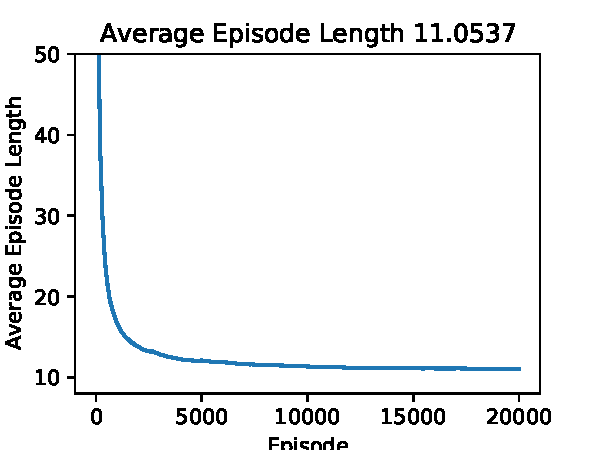
\includegraphics[width=0.6\textwidth]{kings}
	\centering
	\caption{\label{fig:kings} Windy gridworld results with added diagonal moves.}
\end{figure}

\begin{figure}
	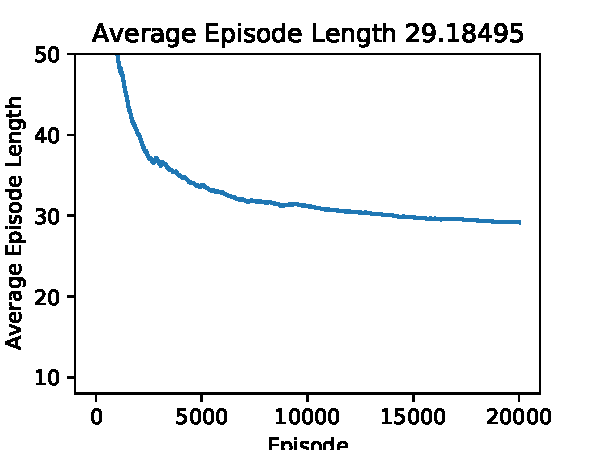
\includegraphics[width=0.6\textwidth]{kings_stochastic}
	\centering
	\caption{\label{fig:kings_stochastic} Windy gridworld results with added noise in the wind. }
\end{figure}

\begin{figure}
	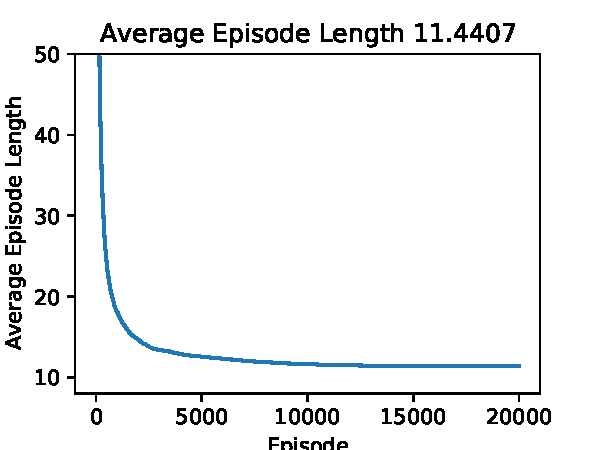
\includegraphics[width=0.6\textwidth]{kings_stationary}
	\centering
	\caption{\label{fig:kings_stationary} Windy gridworld, no noise but allow for staying still.}
\end{figure}

\myq{6.11: Q-Learning}
Q-Learning is an off-policy methods because it learns the action-value function for the \emph{optimal policy} whilst acting with a sub-optimal, behavioural policy. 

\myq{6.12: Sarsa vs Q-Learning}
Suppose \textbf{all} action selection, across both Q-Learning and Sarsa is greedy. Then Sarsa picks the optimal action to perform in a state S, performs this, observes state S'. It then samples the optimal action for S', and uses this Q value for bootstrapping. 

Instead consider Q-Learning. All action selection is greedy, so given state S, we pick the same optimal action as in Sarsa. Similarly, we perform this action, observe the new state and use the optimal action in this state for bootstrapping. 

So yes, in this case, both algorithms are the same. They are however both useless, as they will only update the visited states. 

\myq{6.13: Double Expected Sarsa}
The general algorithm is as follows. 
\begin{algorithm}[H]
	\caption{Double Expected-Sarsa
		\label{alg:double expected sarsa}}
	\begin{algorithmic}[1]
		\Require{
			\textbf{Parameters:} \Statex \hspace{\algorithmicindent} step size $\alpha \in (0, 1]$
			\Statex \hspace{\algorithmicindent} small $\epsilon > 0$ 
		}
		\Statex 
		\Require{
			\textbf{Initialisation:} \Statex \hspace{\algorithmicindent} $Q_1(s, a)$ arbitarily for all $s \in \altmathcal{S}, a \in \altmathcal{A}$ except that $Q_1(\texttt{terminal}, \cdot) = 0$
			\Statex \hspace{\algorithmicindent} $Q_2(s, a)$ arbitarily for all $s \in \altmathcal{S}, a \in \altmathcal{A}$ except that $Q_2(\texttt{terminal}, \cdot) = 0$
		} 
		\Statex
		\Loop{ for each episode}: 
		\State initialise $S$
		\Loop{ for each episode step}:
		\State Choose $A$ using $Q_1(S, \cdot) + Q_2(S, \cdot)$ e.g., $\epsilon$-greedy. \Comment{Off-Policy Method; this is the behavioural policy}
		\State Take action $A$, observe $S', R$
		\If{\texttt{coin-toss} is \texttt{heads}}
			\State derive policy $\pi_1$ from $Q_1$\Comment{e.g. greedy policy yields Q-Learning, $\epsilon$-greedy}
			\Let{$Q_2(S, A)$}{$Q_2(S, A) + \alpha [R + \gamma \sum_{a} \pi_1(a, S')\ Q_2(S', a) - Q_2(S, A)]$}
		\Else
				\State derive policy $\pi_2$ from $Q_2$
				\Let{$Q_1(S, A)$}{$Q_1(S, A) + \alpha [R + \gamma \sum_{a} \pi_2(a, S')\ Q_1(S', a) - Q_1(S, A)]$}
		\EndIf	
		\Let{$S$}{$S'$}
		\EndLoop
		\EndLoop
	\end{algorithmic}
\end{algorithm}
For the specific question, simply substitute in the target epislon greedy policy values i.e., 
\begin{align}
\pi_1(a | S') = \begin{cases}
{\epsilon}/|\altmathcal{A}(S')|,\quad & a \neq \arg\max Q_1(S', a) \\
1 - \epsilon + {\epsilon}/|\altmathcal{A}(S')| , &\text{otherwise}
\end{cases},
\end{align}
and similarly for $\pi_2$. 

\myq{6.14: Afterstates}
In Jack's policy rental, the initial part of the dynamics is known fully i.e., how many cars will move. What is not known is how many cars will arrive or be requested. We can formulate this directly using \emph{afterstates}, where the afterstate is the number of cars at each location \emph{after} cars have been moved from one location to the next. 

This is expected to speed up convergence, for the general reason that we expect afterstates to be useful. There are many state-action pairs which lead to the same afterstate, and thus should have the same value. For example, $(10, 10)$ and moving $2$ cars to give $(8, 12)$ ought to have the same value as being in state $(9, 11)$ and only moving $1$ car. Afterstates add a helpful inductive bias, utilising additional knowledge of the problem, and thus they ought to be helpful. 


\end{document}